\section{The Hash-and-Resubmit Pattern}

We now introduce a novel design pattern for Solidity smart contracts that
results into massive gas optimization due to the elimination of expensive
storage operations.

\textbf{Motivation.}
% This part is maybe too shallow. Consider deleting it. >>>> In the Ethereum
% blockchain, Turing-complete smart contracts were introduced. In order to
% prevent accidental or adversarial DoS phenomena such as infinite loops of
% code, contract invocations are bounded by an amount of gas units~\cite{wood,
% buterin}.  <<<<
It is essential for smart contracts to store data in the blockchain. However,
interacting with the storage of a contract is among the most expensive
operations of the EVM~\cite{wood, buterin}. Therefore, only necessary data
should be stored and redundancy should be avoided when possible. This is
contrary to conventional software architecture, where storage is considered
cheap. Usually, the performance of data access in traditional systems is
related with time. In Ethereum, however, performance is related to gas
consumption. Access to persistent data costs a substantial amount of gas, which
has a direct monetary value. One way to mitigate gas cost of reading variables
from the blockchain is to declare them public.  This leads to the creation of a
\emph{getter} function in the background, allowing free access to the value of
the variable. But this treatment does not prevent the initial population of
storage data, which is significantly expensive for large size of data.
Towards the goal of implementing gas-efficient smart contracts, several
patterns have been proposed~\cite{contract-opt-1, contract-opt-2,
contract-opt-3, contract-opt-4}.

By using the \emph{hash-and-resubmit} pattern, large structures are omitted
from storage entirety, and are contained in memory. When a function call is
performed, the signature and arguments of the function is included in the
transactions field of the body of a block. The contents of blocks are public to
the network, therefore this information is locally available to full nodes. By
simply observing blocks, a node retrieves data sent to the contract by other
users. To interact publicly with this data without the utilization storage, the
node \emph{resends} the observed data to the blockchain. The concept of
resending data is redundant in conventional systems. However, this technique
is very efficient to use in Solidity due to the significantly lower gas cost
of memory operations in relation with storage operations.

\begin{figure*}[h]
    \begin{center} 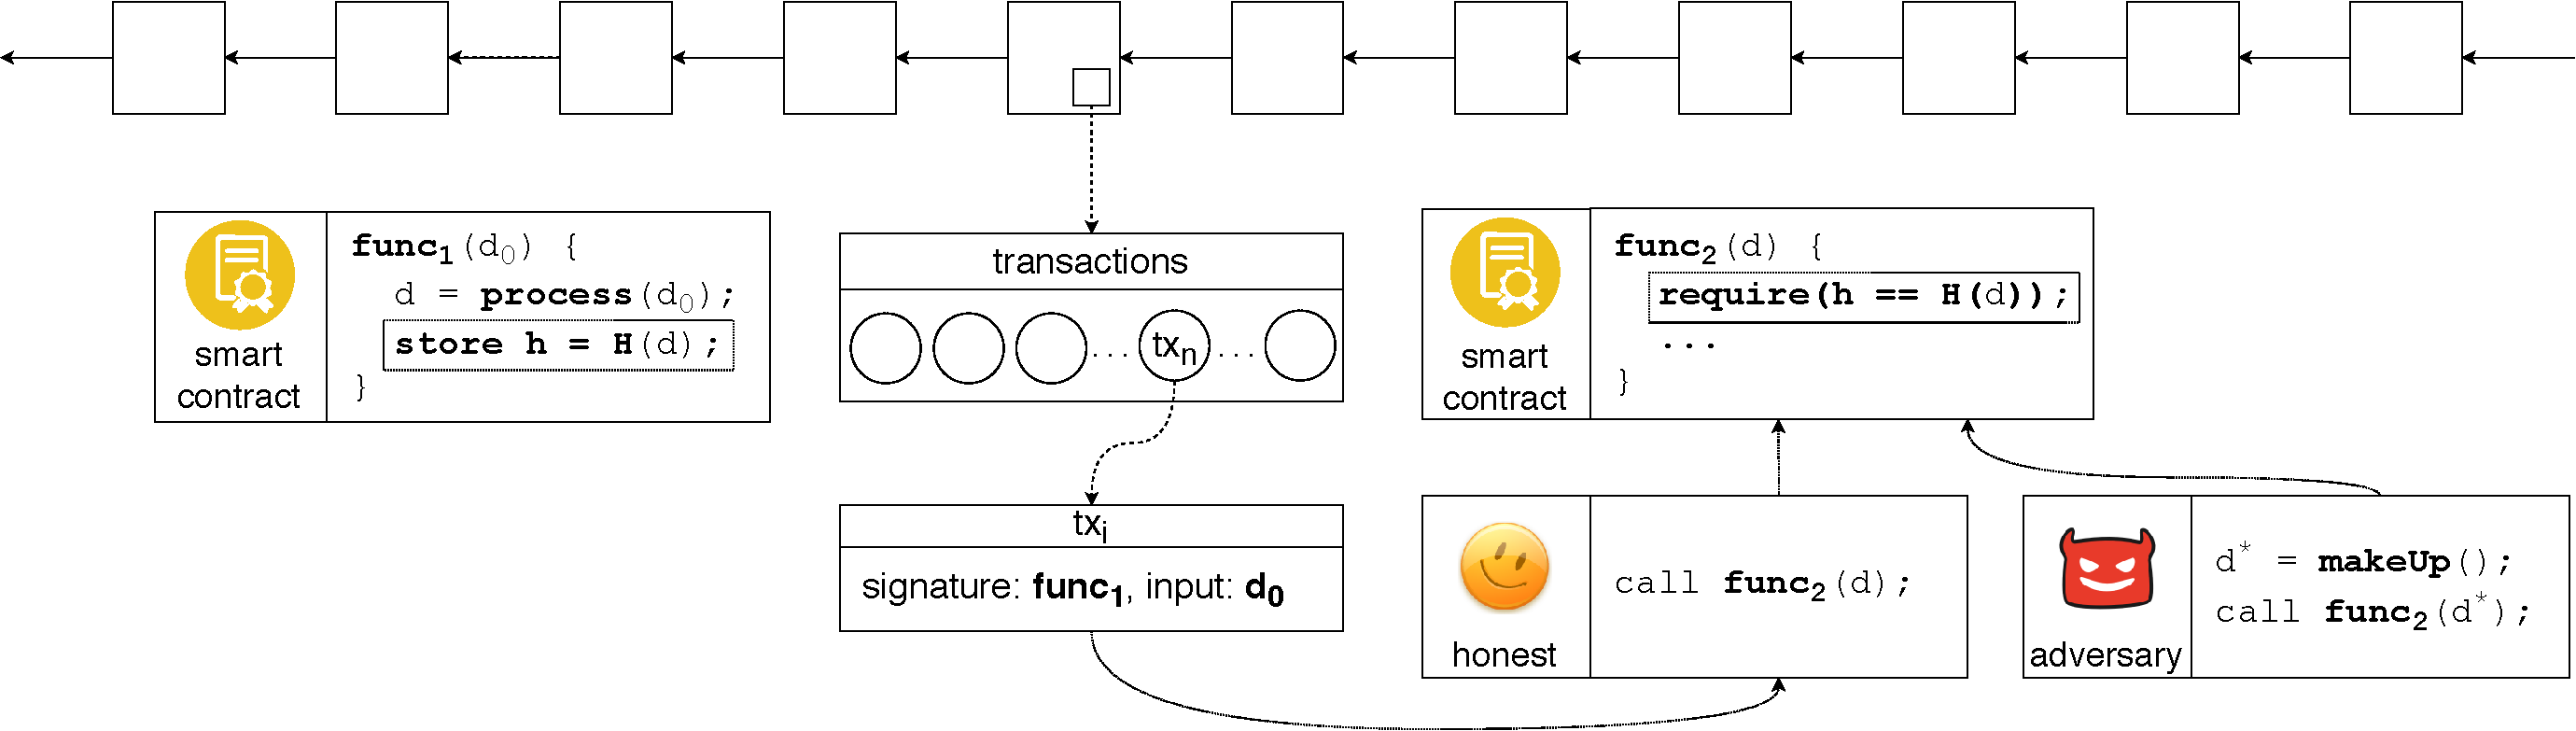
\includegraphics[width=1\textwidth]{figures/har-pattern.pdf}
    \end{center}

    \caption{The \emph{hash-and-resubmit} pattern. In Stage 1, an invoker calls
        \proc$_1$($\data_0$). $\data_0$ is processed on-chain and $\data$ is
        generated. The signature of $\data$ is stored in the blockchain as the
        digest of a hash function \textsf{H}(). In Stage 2, a full node that
        observes invocations of $\proc_1$ retrieves $\data_0$, and generates
        $\data$ by performing the analogous processing on $\data_0$
        \emph{off-chain}. An adversarial observer potentially alters $\data$.
        Finally, in Stage 3, the observer invokes $\proc_2$($\data^*$). In
        $\proc_2$, the validation of $\data$ is performed, reverting the
        function call if the signatures of originally submitted $\data$ does
        not match the signature of $\data^*$. By applying the
        \emph{hash-and-resubmit pattern}, only fixed-size signatures of data
        need to be maintained on the blockchain replacing arbitrarily large
        structures.}

        \label{fig:har-pattern}
\end{figure*}

\noindent
\textbf{Applicability.}
We now list the cases in which the \emph{hash-and-resubmit} pattern is
efficient to use:

The situations in which the \emph{hash-and-resubmit} pattern can be applied are
the following:
\begin{enumerate}
    \item The application is a Solidity smart contract.
    \item Read/write operations are performed in large arrays that exist in
        storage. Rehashing variables of small size may result to negligible
        gain or even performance loss.
    \item The entity that operates on the structures is a full node and
        observes function calls to the smart contract.
\end{enumerate}

\noindent \textbf{Participants and collaborators.} The first participant is the
smart contract $\contract$ that accepts function calls. Another participant is
the invoker $\invoker$, who dispatches a large array $\data_0$ to $\contract$
via a function \texttt{\proc$_1$}($\data_0$). Note that $\data_0$ is
potentially processed in $\proc_1$, resulting to $\data$. The last participant
is the observer $\observer$, who is a full node that observes transactions
towards $\contract$ in the blockchain. This is possible because nodes maintain
the blockchain locally. After observation, $\observer$ retrieves data $\data$.
Since this is an off-chain operation, a malicious $\observer$ potentially
alters $\data$ before interacting with $\contract$. We denote the
potentially modified $\data$ as $\datas$. Finally, $\observer$ acts as an
invoker by making a new call to $\contract$, \texttt{\proc$_2$}($\datas$). The
verification that $\data = \datas$, which is a prerequisite for the secure
functionality of the underlying contract consists a part of the pattern and is
performed in \texttt{\proc$_2$}.

\noindent \textbf{Implementation.} The implementation of this pattern is
divided in two parts. The first part covers how $\datas$ is retrieved by
$\observer$, whereas in the second part the verification of $\data=\datas$ is
realized. The challenge here is twofold:

\begin{enumerate}

    \item Availability: $\observer$ must be able to retrieve $\data$ without
        the need of accessing on-chain data.

    \item Consistency: $\observer$ must be prevented from dispatching $\datas$
        that differs from the originally submitted $\data$.

\end{enumerate}

\noindent
\emph{Hash-and-resubmit} technique is performed in two
stages to face these challenges: (a) the \emph{hash} phase, which addresses
\emph{consistency}, and (b) the \emph{resubmit} phase which addresses
\emph{availability} and \emph{consistency}.

\noindent \textsf{Addressing availability:} During \emph{hash} phase,
$\invoker$ makes the function call \texttt{\proc}$_1$($\data_0$). This
transaction, which includes a function signature (\texttt{\proc$_1$}) and the
corresponding data ($\data_0$), is added in a block by a miner. Due to
blockchain's transparency, the observer of \texttt{\proc}$_1$, $\observer$,
retrieves a copy of $\data_0$, without the need of accessing contract data. In
turn, $\observer$ performs \emph{locally} the same set of on-chain instructions
operated on $\data_0$ generating $\data$. Thus, availability is addressed
through observability.

\noindent \textsf{Addressing consistency} We prevent an adversary $\observer$
from altering $\datas$ by storing the \emph{signature} of $\data$ in contract's
state during the execution of \texttt{\proc$_1$($\data$)} by $\invoker$. In the
context of Solidity, a signature of a structure is the digest of the
structure's \emph{hash}. The pre-compiled \texttt{sha256} is convenient to use
in Solidity, however we can make use of any cryptographic hash function
\textsf{H()}: \[\textsf{hash} \gets \textsf{H}(\textsf{d})\] Then, in
\emph{rehash} phase, the verification is performed by comparing the stored
digest of $\data$ with the digest of $\datas$.
\[\textsf{require}(\textsf{hash} = \texttt{H}(\datas))\] \noindent In Solidity,
the size of digests is 32 bytes. To persist such a small value in contract's
memory only adds a constant, negligible cost overhead.

We illustrate the application of the \emph{hash-and-resubmit} pattern in
Figure~\ref{fig:har-pattern}.

\noindent \textbf{Sample.} We now demonstrate the usage of the
hash-and-resubmit pattern with a simplistic example. We create a smart contract
that orchestrates a game between two players, $\pla$ and $\plb$. The winner is
the player with the most valuable array. The interaction between players
through the smart contract is realized in two phases: (a) the submit phase and
(b) the contest phase.

\noindent \textsf{Submit phase:} $\pla$ submits an N-sized array, $\arra$ and
becomes the $\holder$ of the contract.

\noindent \textsf{Contest phase:} $\plb$ submits $\arrb$. If
\textsf{compare}($\arrb$, $\arra$) is true, then the $\holder$ of the contract
changes to $\plb$. We provide a simple implementation for \textsf{compare()},
but we can consider any notion of comparison, since the pattern is abstracted
from such implementation details.

We make use of the \emph{hash-and-resubmit} pattern by prompting $\plb$ to
provide \emph{two} arrays to the contract during contest phase: (a) $\arras$,
which is the originally submitted array by $\pla$, possibly modified by $\plb$,
and (b) $\arrb$, which is the contesting array.

We provide two implementations of the above described game.
In Algorithm~\ref{alg:game-storage} we display the storage implementation,
while in Algorithm~\ref{alg:game-memory} we show the implementation
embedding the \emph{hash-and-resubmit} pattern.

\begin{algorithm}
    \caption{\label{alg:game-storage}\textsf{best array} using storage}
    \begin{algorithmic}[1]

    \Contract{best-array}
        \State{$\textsf{best} \gets \emptyset$;
               $\textsf{holder} \gets \emptyset$}
        \Function{\sf submit}{$a$}
        \State \textsf{best} $\gets a$
            \Comment{array saved in storage}
            \State \textsf{holder $\gets$ msg.sender}
        \EndFunction

        \Function{\sf contest}{$a$}
            \State \textsf{require}(\textsf{compare}($a$))
            \State \textsf{holder} $\gets$ \textsf{msg.sender}
        \EndFunction

        \Function{\sf compare}{$a$}
            \State \textsf{require}($|a|$ $\geq$ $|$\textsf{best}$|$)
            \For{$i$ \textbf{in} $|$\textsf{best}$|$}
            \State \textsf{require}($a[i]$ $\geq$ \textsf{best}[i])
            \EndFor
            \State \Return{true}
        \EndFunction
        \EndContract
        \vskip8pt
    \end{algorithmic}
\end{algorithm}

\begin{algorithm}
    \caption{\label{alg:game-memory}\textsf{best array} using hash-and-resubmit pattern}
    \begin{algorithmic}[1]
        \Contract{best-array}
        \State{$\textsf{hash} \gets \emptyset$;
               $\textsf{holder} \gets \emptyset$}

        \Function{\sf submit}{$\arra$}
        \State $\textsf{hash} \gets \textsf{H}(\arra)$
            \Comment{hash saved in storage}
            \State \textsf{holder} $\gets$ \textsf{msg.sender}
        \EndFunction

    \Function{\sf contest}{$\arra^*$, $\arrb$}
    \State \textsf{require}(\textsf{hash256}($\arra^*$) $=$ $hash$)
        \Comment{validate $\arra^*$}
        \State \textsf{require}(\textsf{compare}($\arra^*$, $\arrb$))
        \State \textsf{holder} $\gets$ \textsf{msg.sender}
    \EndFunction
    \Function{\sf compare}{$\arra^*$, $\arrb$}
        \State \textsf{require}($|\arra^*|$ $\geq$ $|\arrb|$)
        \For{$i$ \textbf{in} $|\arra^*|$}
            \State \textsf{require}($\arra^*[i] \geq \arrb[i]$)
        \EndFor
    \EndFunction
    \State \Return{true}
    \EndContract
    \vskip8pt
    \end{algorithmic}
\end{algorithm}


\noindent \textbf{Gas analysis.} The gas consumption of the two above
implementations is displayed in Figure~\ref{fig:har-example}. By using the
\emph{hash-and-resubmit} pattern, the aggregated gas consumption for
\textsf{submit} and \textsf{contest} is decreased by 95\%. This significantly
affects the efficiency and applicability of the contract. Note that, the
storage implementation exceeds the Ethereum block gas limit\footnote{As of July
2020, the Ethereum block gas limit approximates 10,000,000 gas units} for
arrays of size 500 and above, contrary to the optimized version, which consumes
approximately only $1/10^{th}$ of the block gas limit for arrays of 1000
elements.

\begin{figure}[h!]
\begin{center}
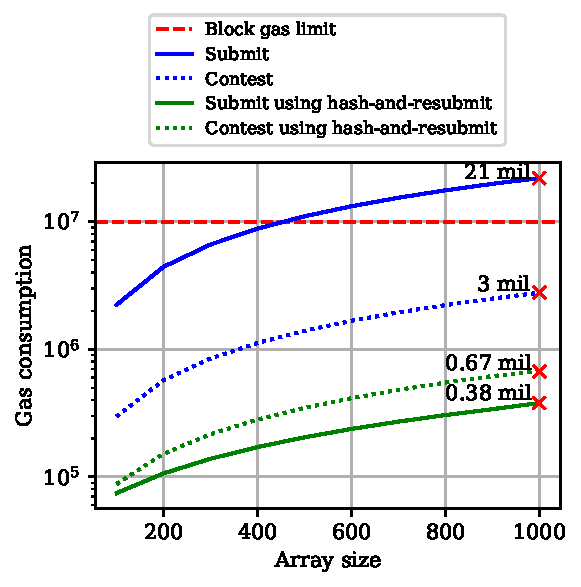
\includegraphics[width=1 \columnwidth]{figures/har-example.pdf}
\end{center}
\caption{Gas-cost reduction using the \emph{hash-and-resubmit} pattern. By
    avoiding gas-heavy storage operations, the aggregated cost of
    \textsf{submit} and \textsf{contest} is decreased significantly by 95\%.}
\label{fig:har-example}
\end{figure}


\noindent \textbf{Variations.}

% Now consider a variation of the above game, in
% which $\pla$ calls \texttt{\proc$_1$(}$\arra$\texttt{)}, and then calls
% \texttt{pickSpan(}$m, n$\texttt{)} that determines the span of $\arra$ which
% can be contested. In reality, $\plb$ only needs to re-send $\arras[m:n]$ in
% order to perform the comparison $\arra[m:n] < \arrb$. However, the digest of
% $\arra$ is calculated by hashing the entire structure. Therefore, the
% $resubmit$ phase cannot be successfully performed by rehashing $\arras[m:n]$,
% because \texttt{H(}$\arra$\texttt{)} $\ne$ \texttt{H(}$\arra[m:n]$\texttt{)}.

In order to enable selective dispatch of a segment of interest, different
hashing schemas can be adopted, such as Merkle Trees (ref) and Merkle Mountain
Ranges (ref). In this variation of the pattern, which we term
\emph{merkle-hash-and-resubmit}, the signature of an array $\textsf{D}$ is
Merkle Tree Root (MTR). In \emph{resubmit} phase, $\textsf{D}[m:n]$ is
dispatched, accompanied by the siblings that reconstruct the MTR of
$\textsf{D}$.

\begin{figure*}[h]
    \begin{center}
        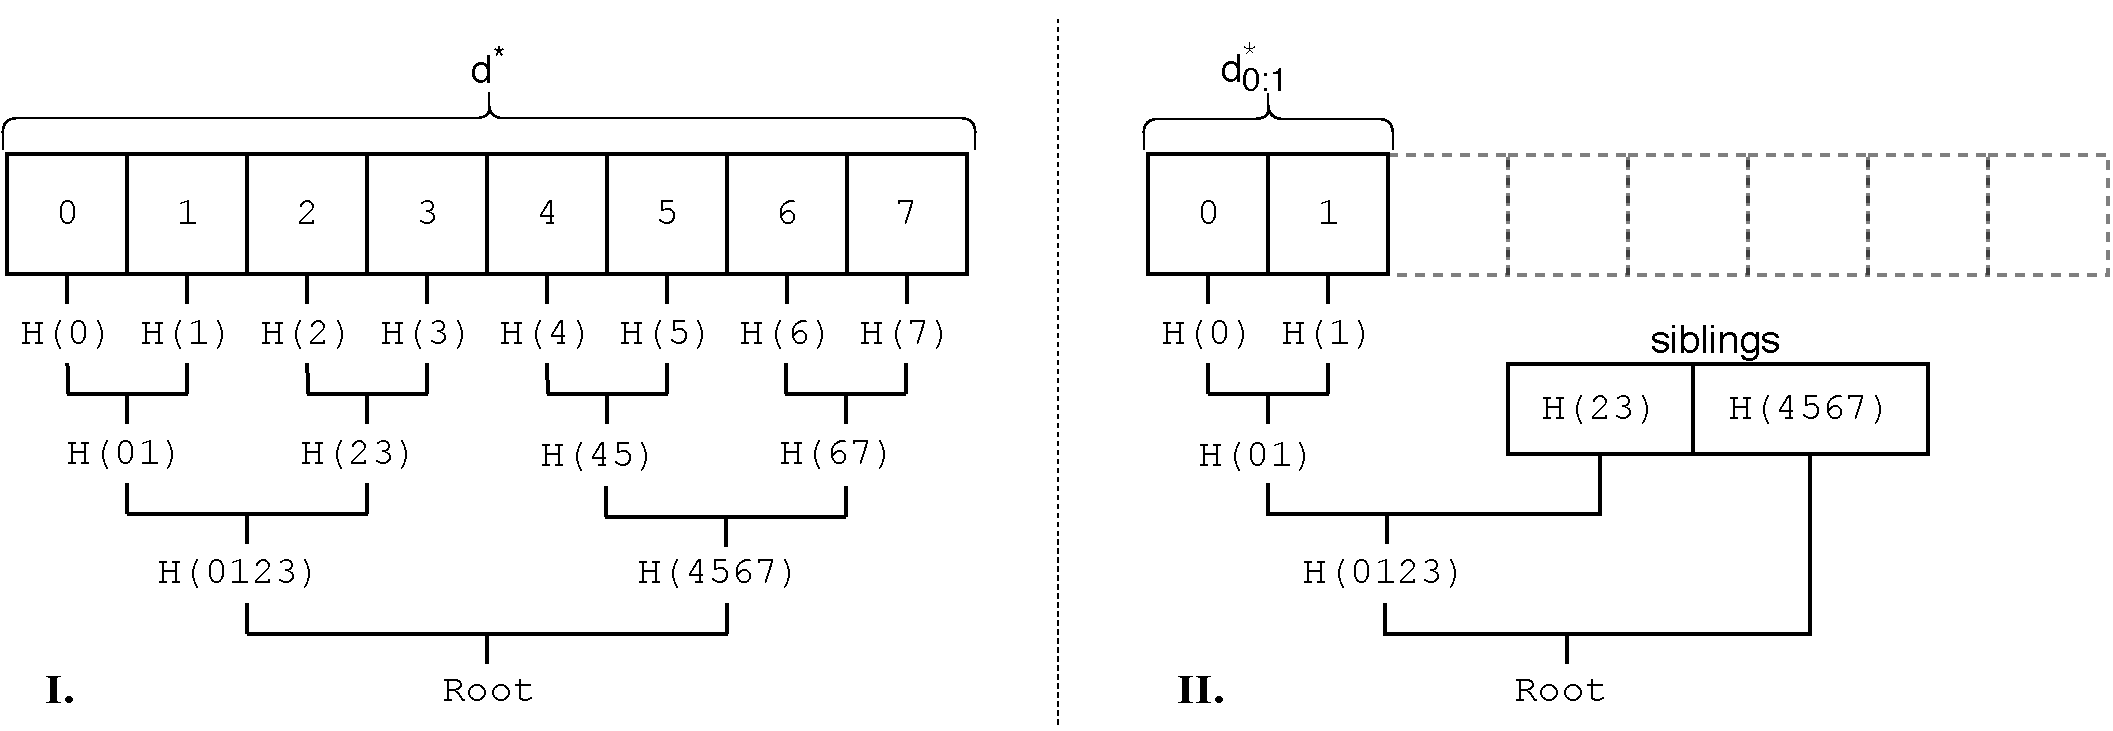
\includegraphics[width=0.8\textwidth]{figures/merkle-har.pdf}
    \end{center}
    \caption{\textbf{I.} The calculation of root in \emph{hash} phase.
    \textbf{II.} The verification of the root in \emph{resubmit} phase.
    \textsf{H}($k$) denotes the digest of element $k$. \textsf{H}($kl$) denotes the
    result of \textsf{H}(\textsf{H}($k$) $|$ \textsf{H}($l$))
}
    \label{fig:merkle-har}
\end{figure*}

This variation of the pattern removes the burden of sending redundant data,
however it implies on-chain construction and validation of the Merkle
construction. In order to construct a MTR for an array $\data$,
$|\data|$ hashes are needed for the leafs of the MT, and $|\data| -
1$ hashes are needed for the intermediate nodes. For the verification, the
segment of interest $\data[m:n]$ and the siblings of the MT are hashed.
The size of siblings is approximately $log_2(|\data|)$. The process of
constructing and verifying the MTR is displayed in Figure
~\ref{fig:merkle-har}.

In Solidity, different hashing operations vary in cost. An invocation of
\textsf{sha256}($\data$), copies $data$ in memory, and then the
\emph{CALL} instruction is performed by the EVM that calls a pre-compiled
contract. In the current state of the EVM, \emph{CALL} costs 700 gas units, and
the gas paid for every word when expanding memory is 3 gas units~\cite{wood}.
Consequently, the expression $1 \times \textsf{sha256}(\data)$ cost less that
$|\data| \times $\textsf{sha}(1) operations. A different cost policy applies
for \textsf{keccak}~\cite{keccak} hash function, where hashing costs 30 gas
units plus 6 additional gas far each word for input data~\cite{wood}. The usage
of \textsf{keccak} dramatically increases the performance in comparison with
\textsf{sha256}, and performs better than plain rehashing if the product of
on-chain processing is sufficiently larger that the originally dispatched data.
Costs of all related operations are listed in Table~\ref{tab:operations-gas}.

The merkle variation can be potentially improved by dividing $\data$ in larger
chunks than 1 element. We leave this analysis for future work.

\begin{table}[!h]
\begin{tabular}{|c|c|}
\hline
\textbf{Operation} & \textbf{Gas cost} \\ \hline
\textsf{load}($\data$)            & $ \data_{bytes} \times 68 $          \\ \hline
\textsf{sha256}($\data$)          & $\data_{words} \times 3 + 700 $     \\ \hline
\textsf{keccak}($\data$)          & $\data_{words} \times 6 + 30 $      \\ \hline
\end{tabular}
\caption{Gas cost of EVM operations as of June 2020.}
\label{tab:operations-gas}
\vspace*{-5mm}
\end{table}


In Table~\ref{tab:har-vs-mhar} we display the operations needed for hashing and
verifying the underlying data for both variations of the pattern as a function
of data size. In Figure~\ref{fig:har-vs-mhar} we demonstrate the gas
consumption for dispatched data of 10KB, and varying size of on-chain
process product.

\newcommand{\mydata}{\data}

\begin{table}[h]
\begin{tabular}{|c|c|c|}
\hline
\textbf{\begin{tabular}[c]{@{}c@{}}phase per\\variance\end{tabular}} &
\textbf{\begin{tabular}[c]{@{}c@{}}plain hash\\and resubmit\end{tabular}} &
\textbf{\begin{tabular}[c]{@{}c@{}}merkle hash\\ and resubmit\end{tabular}} \\ \hline
\textbf{hash} &
\textsf{H}($\mydata$) &
\begin{tabular}[c]{@{}c@{}}
    \textsf{H}($\mydata_{elem}$) $\times\ |\mydata|$ \\ \textsf{H}(digest)
$\times\ (|\mydata|-1)$

\end{tabular} \\ \hline
\textbf{resubmit} &
\textsf{load}($\mydata$) + \textsf{H}($\mydata$) &
\begin{tabular}[c]{@{}c@{}}
    \textsf{load}($\mydata[m{:}n])$ + \\
    \textsf{load}($siblings$) + \\
    \textsf{H}($\mydata[m{:}n])$ + \\
    \textsf{H}($digest$)$\times |siblings|$
\end{tabular} \\ \hline
\end{tabular}

\caption{Summary of operations for \emph{hash-and-resubmit} pattern variations.
$\mydata$ is the product of on-chain operations and $\mydata_{elem}$ is an
element of $\mydata$. \textsf{H} is a hash function, such as \textsf{sha256}
or \textsf{keccak}, $digest$ is the product of \textsf{H}(.) and $siblings$ are
the siblings of the Merkle Tree constructed for $\mydata$.
}

\label{tab:har-vs-mhar}
\vspace*{-10mm}
\end{table}


\begin{figure}[h]
    \begin{center}
        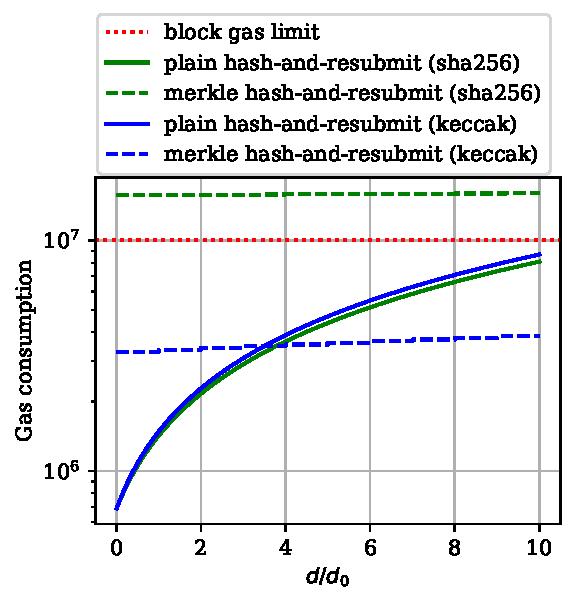
\includegraphics[width=1\columnwidth]{figures/har-vs-mhar.pdf}
    \end{center}
    \caption{Trade-offs between \emph{hash-and-resubmit} variations. In the
    vertical axis the gas consumption is displayed, and in vertical axis the
    size of $\data$ as a function of $\data_0$. The size of $d_0$ is 10KB
    bytes, and the hash function we used is pre-compiled \texttt{sha256}.}
    \label{fig:har-vs-mhar}
\end{figure}

\noindent \textbf{Consequences.} The most obvious consequence of applying the
\emph{hash-and-resubmit} pattern variations is the circumvention of storage
structures, a benefit that saves a substantial amount of gas, especially in the
cases where these structures are large. To that extend, smart contracts that
exceed the Ethereum block gas limit become practical. Furthermore, the pattern
enables off-chain transactions, significantly improving the performance of
smart contracts.

\noindent \textbf{Known uses.} To our knowledge, we are the first to combine
the notion of the transparency of the blockchain with data structures
signatures to eliminate storage variables from Solidity smart contracts by
resubmitting data.

\noindent \textbf{Enabling NIPoPoWs.} We now present how the
\emph{hash-and-resubmit} pattern can used in the context of the NIPoPoW
superlight client. Similar to the aforementioned example, the NIPoPoW verifier
adheres to a submit-and-contest-phase schema, and the inputs of the functions
are arrays that are processed on-chain.

In \emph{submit} phase, a \emph{proof} is submitted, which can be contested by
another user in \emph{contest} phase. The user that initiates the contest,
monitors the traffic of the smart contract~\cite{nipopows}. The input of
\textsf{submit} function includes the submit proof ($\pis$) that indicates the
occurrence of an \emph{event} ($e$) in the source chain, and the input of
\textsf{contest} function includes the contesting proof ($\pic$). A successful
contest of $\pis$ is realized when $\pic$ has a better score. The score
evaluation process is irrelevant to the pattern and remains unchained. The size
of proofs is dictated by the value $m$. We consider $m$ = 15 sufficiently
secure.

In previous work~\cite{gglou}, NIPoPoW proofs are maintained on-chain,
resulting to extensive storage operations that limit the applicability of the
contract considerably. In Algorithm~\ref{alg:har-nipopow} we show how
hash-and-resubmit pattern is embedded into the NIPoPoW client. In
Figure~\ref{fig:har-nipopow}, we display how results of the
\emph{hash-and-resubmit} implementation differentiate from previous work for
the aggregated cost of \emph{submit} and \emph{contest} phases.  We observe
that by using the \emph{hash-and-resubmit} pattern, we achieve to increase the
performance of the contract 40\%. This is a decisive step towards creating a
practical superlight client.

\newcommand{\genesis}{\textsf{G}}

\begin{algorithm}
    \label{alg:har-nipopow}
    \caption{The \textsf{NIPoPoW} client using hash-and-resubmit pattern}
    \begin{algorithmic}[1]

    \Contract{crosschain}
    \State $\textsf{events} \gets \bot;$ $\genesis \gets \bot$
    \Function{\sf initialize}{$\genesis_{remote}$}
        \State \genesis $\gets \genesis_{remote}$
    \EndFunction
    \Function{\sf submit}{$\pis$, $e$}
        \State \textsf{require}($\pis$[0] = $\genesis$)
        \State \textsf{require}($\textsf{events$[e]$} = \bot$)
        \State \textsf{require}($\textsf{valid-interlink}(\pi)$)
        \State \textsf{DAG} $\gets$ \textsf{DAG} $\cup$ $\pis$
        \State \textsf{events$[e]$.hash} $\gets$ \textsf{H}($\pis$)
        \Comment{enable pattern}
        \State \textsf{ancestors} $\gets$ \textsf{find-ancestors()}
        \State \textsf{events$[e]$.pred} $\gets$
            \textsf{evaluate-predicate}(\textsf{ancestors}, e)
        \State \textsf{ancestors} $=$ $\bot$
    \EndFunction
    \Function{\sf contest}{$\pisa$, $\pic$, $e$}
        \Comment{provide proofs}
        \State \textsf{require}(\textsf{events$[e]$.hash} $=$ \textsf{H}($\pisa$))
        \Comment{verify $\pisa$}
        \State \textsf{require}($\pic$[0] = $\genesis$)
        \State \textsf{require}(\textsf{events}$[e]$ $\ne$ $\bot$)
        \State \textsf{require}(\textsf{valid-interlink}($\pi_{cont}$))
        \State $lca$ = \textsf{find-lca}($\pisa$, $\pic$)
        \State \textsf{require}(\textsf{score}($\pic[:lca]$)
            $>$ \textsf{score}($\pisa[:lca]$))
        \State \textsf{DAG} $\gets$ \textsf{DAG} $\cup$ $\pic$
        \State \textsf{ancestors} $\gets$ \textsf{find-ancestors}(\textsf{DAG})
        \State \textsf{events$[e]$.pred} $\gets$
            \textsf{evaluate-predicate}(\textsf{ancestors}, $e$)
        \State \textsf{ancestors} $=$ $\bot$
    \EndFunction
    \EndContract
    \vskip8pt
    \end{algorithmic}
\end{algorithm}



\begin{figure}[!h]
    \begin{center}
        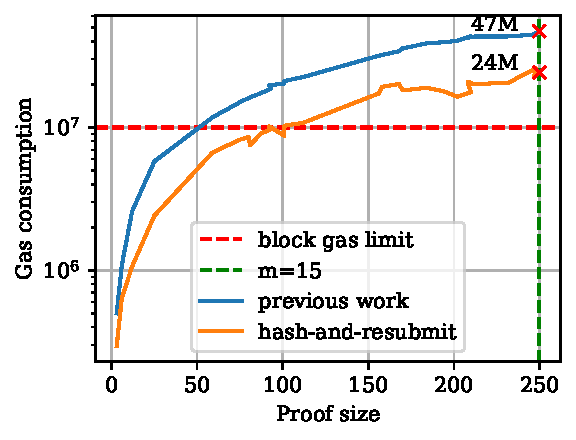
\includegraphics[width=1\columnwidth]{figures/har-nipopows.pdf}
    \end{center}
    \caption{Performance improvement using hash-and-resubmit pattern in
    NIPoPoWs related to previous work for a secure value of $m$. The gas
    consumption decreased by approximately 40\%.}
    \label{fig:har-nipopow}
\end{figure}
